\section{Projektplanung}

Die Projektplanung wurde anhand der vorgegebenen Abgabetermine durchgeführt.
Da es vier Abgabetermine gibt, wurde das Projekt in vier Sprints aufgeteilt, die jeweils mit einem Meilenstein enden. 

\subsection{Risikobewertung}

Die Risiken des Projektes sind gesammelt und bewertet worden. Pro Risiko wurden Massnahmen zur Prävention und zur Mitigation gesammelt. Die Bewertung wurde durchgeführt vor dem Umsetzen der Massnahmen (V.) und nachher (N.).
Zusätzlich zu den definierten Massnahmen sollen mithilfe von Prototypen so viele Risiken wie möglich, so gut wie möglich vermindert werden. 

\begin{table}[H]
\centering
\small
\begin{tabularx}\textwidth{|c | X | X | X | c | c|}
\hline
  \textbf{Nr} & \textbf{Beschreibung} & \textbf{Prävention} & \textbf{Mitigation} & \textbf{V.} & \textbf{N.} \\
  \hline
    1&Hindernisse werden nicht erkannt. &Mit vielen Bildern trainieren.& Distanzsensor; Roboter fährt zurück.&20&5 \\
  \hline
      2&Knoten werden nicht erkannt. &Viele Bilder in verschiedenen Situationen machen, um zu trainieren.&Linien werden erkannt und Roboter orientiert sich daran.&20& 12\\
  \hline
      3&4 Minuten reichen nicht. &Testdurchfläufe in realistischen Umgebungen.&&8&4 \\
  \hline
      4& 1 Minute reicht nicht zum Aufbau.& Testdurchfläufe und einfaches Interface.&Zufälliges Ziel wird gewählt von SW.&5&3 \\
  \hline
      5&Bodenfugen werden als Linie erkannt. & Testdurchfläufe in realistischen Umgebungen.&Kamera hilft Linien zu erkennen, hilft Roboter gerade zu stellen.&15&4 \\
  \hline
      6& Liniensensor fehlerhaft. &Sichere Implementation mit Tests.& Encoder Motoren.&8&3 \\
  \hline
      7& Ein Objekt wird fehlerhaft gedeutet und falsche Wege werden intern entfernt. &Knoten erkennen und nicht nur Hindernisse.&Roboter ist schnell genug und hat einen Trial \& Error Modus.&16&6 \\
  \hline
      8&Hindernisse werden beim Anheben verschoben. &Robuste Greifmethode waehlen und testen.&&12&8 \\
  \hline
      9&Überstrom bei blockierten Motoren. &Endschalter, Stromsensoren.&Abschalten bevor Bauteile beschädigt.&10&5 \\
  \hline
      10&Ungenaue Abfahrtsituation vom Knoten, Fahrzeug fährt von der Linie weg. &Liniensensor als Unterstützung, Kamera prueft Linie&Korrigieren falls nötig.&15&5 \\
  \hline
      11&Die Kamera liefert unscharfe oder verzerrte unbrauchbare Bilder. &Verwendung von Kameras mit hoher Auflösung.&Falls Bilder unscharf sind, Roboter anhalten und neue Bilder aufnehmen.&12&6 \\
  \hline
      12& Der Roboter wählt einen falschen Pfad, weil die Hinderniserkennung fehlerhaft ist.&Optimierung der Hinderniserkennung.&Roboter bei Fehlverhalten anhalten und zurücksetzen in vorherigen Zustand. Roboter ist schnell.&12& 6\\
  \hline
      13&Ein Softwarefehler führt zu einem Absturz während der Laufzeit, wodurch der Roboter stoppt oder Fehlfunktionen aufweist. &Exception Handling und umfangreiche Tests unter verschiedenen Bedingungen.&Automatischer SW-Neustart, Wiederaufnahme des letzten bekannten Zustands.&15&4 \\
  \hline
      14&Ein Software-Update führt zu neuen Fehlern oder ist nicht kompatibel mit der aktuellen Hardware. &Gründliche Tests vor dem Rollout eines Updates.&Möglichkeit, schnell zur vorherigen stabilen Version zurückzukehren.&6&2 \\
  \hline
      15&Akkustand ist zu niedrig bei Start des Laufes. & Anzeige des Akkustandes. Leicht austauschbarer Akku. Akku aufladen.&Ein zweiter Akku, der voll aufgeladen ist.&5& 1\\
  \hline
      16&Personenausfall durch Krankheit oder Unfall. &&Stellvertretungen und virtuelle Kommunikation.&6& 3\\
  \hline
      17&Datenkorruption. &&Regelmässige Backups.&4& 1\\
  \hline



\end{tabularx}
\caption{Risiken}
\label{table:risks}
\end{table}

Alle Risiken wurden bewertet anhand der Wahrscheinlichkeit und der Auswirkung. Dies ist ersichtlich aus dieser Grafik.

\begin{figure}[H]
\centering
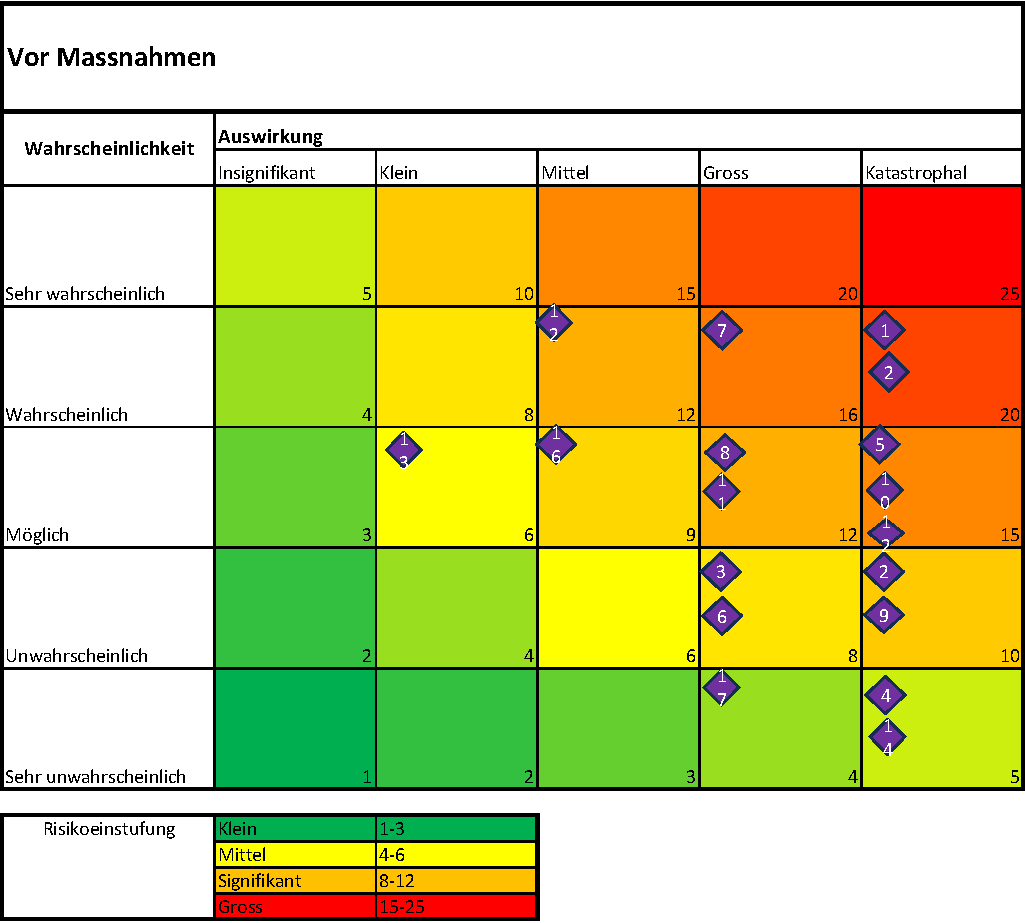
\includegraphics[width=\textwidth -40mm]{assets/Risikoanalyse-vorher.pdf}
\caption{Risikoanalyse vor Massnahmen}
\label{fig:risk-before}
\end{figure}

Dieselbe Matrix wurde erstellt für die Risiken nach den definierten Massnahmen.

\begin{figure}[H]
\centering
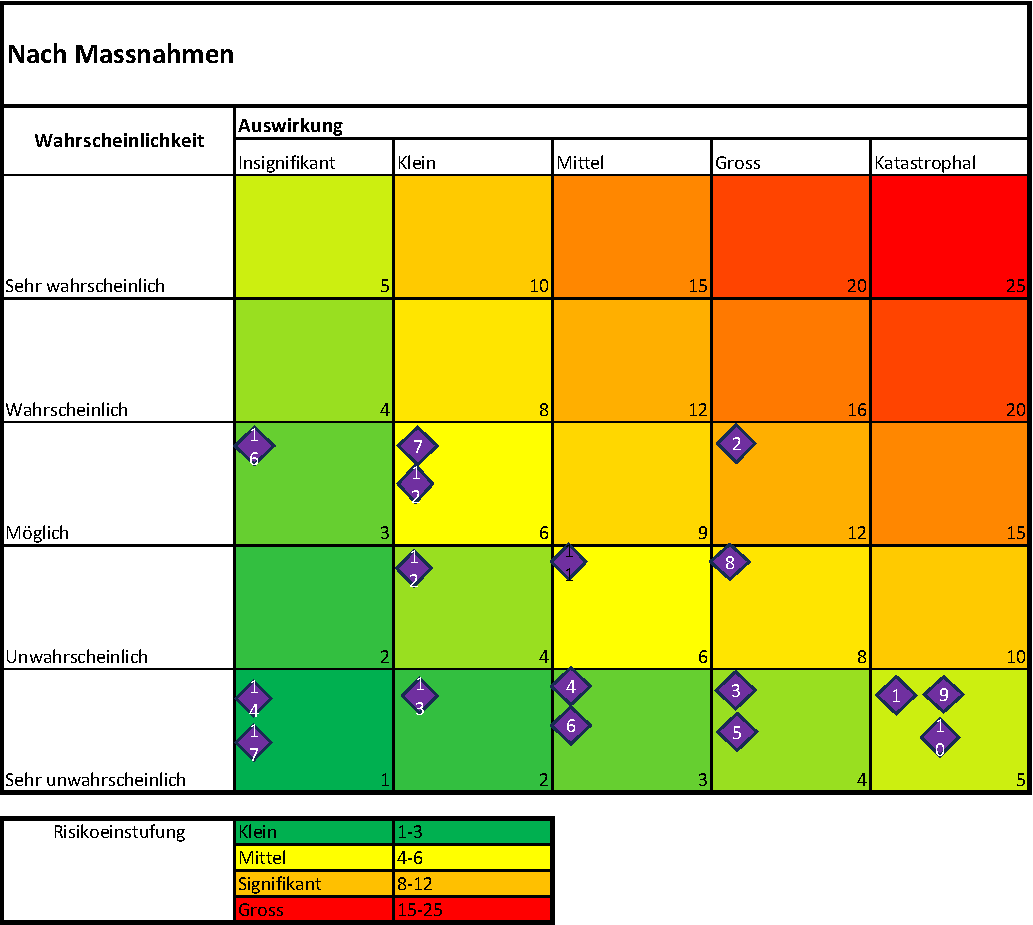
\includegraphics[width=\textwidth -40mm]{assets/Risikoanalyse-nachher.pdf}
\caption{Risikoanalyse nach Massnahmen}
\label{fig:risk-after}
\end{figure}

Aus der Risikomatrix nach den Massnahmen geht hervor, dass die grössten Risiken, die beim Entwickeln des Roboters berücksichtigt werden müssen die folgenden drei Risiken sind:

\begin{itemize}
    \item Risiko 2: Knoten werden nicht erkannt.
    \item Risiko 7: Ein Objekt wird fehlerhaft gedeutet und falsche Wege werden intern entfernt.
    \item Risiko 12: Der Roboter wählt einen falschen Pfad, weil die Hinderniserkennung fehlerhaft ist.
\end{itemize}


\newpage
\subsection{Projektplan}

Der Projektplan in Tabelle \ref{table:projektplan} zeigt die Meilensteine, die zu erreichen sind.
Die Meilensteine sind die einzelnen Testatabgaben.
Die abzugebenden Dokumente pro Testat bilden die einzelnen Sprintziele.

\begin{table}[h!]
\centering
\begin{tabular}{|l  l l|}
\hline
  \textbf{Meilenstein} & \textbf{Datum} & \textbf{Beschreibung} \\
  \hline
  Meilenstein 1  & 04. Oktober 2024 & \makecell{Projektplan, Skizzierung der Aufgabenstellung,\\ Technologierecherche, Anforderungsliste}\\
  \hline
  Meilenstein 2  & 01. November 2024 & \makecell{Evaluation der Lösungsprinzipien, Auswahl der\\ optimalen Lösungeskombinationen}\\
  \hline
  Meilenstein 3  & 06. Dezember 2024 & \makecell{Freigabe des Gesamtkonzepts, Simulator Wegplanung, \\Dokumentation zu 80\% fertiggstellt}\\
  \hline
  Meilenstein 4  & 10. Januar 2025 & \makecell{Schlussbereicht, Präsentation}\\
  \hline
\end{tabular}
\caption{Projektplan}
\label{table:projektplan}
\end{table}

\subsection{Backlog}

Der Backlog dient als zentrales Planungselement.
In diesem Projekt sind die einzelnen Meilensteine vorgegeben. Aus diesem Grund wurden bereits zu Beginn alle Sprints geplant und der ganze Product Backlog wurde in Sprintbacklogs aufgeteilt. Nach Erreichen eines Meilensteins wird ein Ausblick auf den nächsten Sprint durchgeführt, um allfällige Anpassungen an dem Sprintbacklog vorzunehmen.

\subsection{Sprintplanung}

In den folgenden Kapiteln wurden für jeden Sprint Sprintziele definiert und ein Sprintbacklog erstellt. Für den Sprintbacklog wurden die einzelnen Meilensteine aus dem Projektplan in Epics\footnote{https://www.atlassian.com/agile/project-management/epics} beschrieben. Zu den Epics wurden User Stories erstellt. Der Aufwand der einzelnen Stories wurde mit T-Shirt Grössen geschätzt. Die einzelnen T-Shirt Grössen werden wie folgt in eine Zeitdauer umgerechnet:

\begin{table}[h!]
\centering
\begin{tabularx}\textwidth{|X | X |}
\hline
  \textbf{Grösse} & \textbf{Dauer} \\
  \hline
  S  & 4h - 2d \\
  \hline
  M  & 2d - 5d\\
  \hline
  L  & 5d+\\
  \hline
\end{tabularx}
\caption{T-Shirt Grössen}
\label{table:t-shirt}
\end{table}


\newpage
\subsubsection{Sprint 1: 20. September 2024 - 04. Oktober 2024}

\textbf{Sprintziel:}
\begin{itemize}
    \item Projektplan erstellt
    \item Aufgabenstellung skizziert
    \item Andorderungsliste erstellt
    \item Technologierecherche
\end{itemize}

\textbf{Sprintbacklog:} Der Sprintbacklog von Sprint 1 ist in Tabelle \ref{table:sprint1-backlog} dargestellt.

\begin{table}[H]
\centering
\small
\begin{tabularx}{\textwidth}{|l|l|X|c|}
\hline
  \textbf{Nr.} & \textbf{Titel} & \textbf{Beschreibung} & \textbf{Size}\\
  \hline
  1  & \textbf{Projektorganisation definieren} &&\\
  \hline
  1.1  & Rollendefinition & Die Rollen Projektleiter und Werkstattverwantwortliche werden definiert. & S\\
  \hline
  1.2 & Datenaustausch definieren & Zentrale Datenablage und Kommunikationsschnittstellen definieren.& S\\
  \hline
  1.3 & Ziele definieren & Definieren, wie wir uns den Roboter vorstellen. & S\\
  \hline
  1.4 & Vorgehen definieren & Geeignete Projektmethode wird gewählt. & S\\
  \hline
    1.5 & Risikomatrix erstellen & Risiken werden gesammelt und bewertet. & M\\
  \hline
  2 & \textbf{Aufgabenstellung klären} && \\
  \hline
  2.1 & Anforderungsliste erstellen & Anforderungen, die der Roboter erfüllen muss sammeln& M \\
  \hline
  2.2 & Aufgabenstellung skizzieren & Modellierunge der Aufgabe zum Verständnis. & S \\
  \hline
  3 & \textbf{Projektplanung} && \\
  \hline
  3.1 & Projektplan erstellen & Meilensteine definieren. & S \\
  \hline
  3.2 & Backlog erstellen & Product Backlog für alle Sprints erstellen. & M \\
  \hline
  4 & \textbf{Lösungsvarianten erarbeiten} && \\
  \hline
  4.1 & Teilfunktionen finden & Roboter in Teilfunktionen aufteilen & S \\
  \hline
  4.2 & Technologierecherche & Recherche zu den einzelnen Teilfunktionen  durchführen. & L\\
  \hline
 
\end{tabularx}
\caption{Sprint 1 Backlog}
\label{table:sprint1-backlog}
\end{table}

\newpage
\subsubsection{Sprint 2: 04. Oktober 2024 - 01. November 2024}

\textbf{Sprintziel:}
\begin{itemize}
    \item Evaluation der Lösungsprinzipien
    \item Auswahl der optimalen Lösungeskombinationen
\end{itemize}

\textbf{Sprintbacklog:} Der Sprintbacklog von Sprint 2 ist in Tabelle \ref{table:sprint2-backlog} dargestellt.


\begin{table}[H]
\centering
\small
\begin{tabularx}{\textwidth}{|l|l|X|c|}
\hline
  \textbf{Nr.} & \textbf{Titel} & \textbf{Beschreibung} & \textbf{Size}\\
  \hline
  1  & \textbf{Evaluation Lösungsvarianten} &&\\
  \hline
  1.1  & Workshop Auschlusskriterien & Brainstorming, um herauszufinden, was wir nicht wollen, um Technologien auszuschliessen. & S\\
  \hline
  1.2 & Erste Aussortierung & Lösungsvarianten aussortieren ahhand Auschlusskriterien. & M\\
  \hline
  1.3 & Morphologischer Kasten & Morphologischer Kasten erstellen, um Lösungskombinationen zu ermitteln. & L\\
  \hline
  1.4 & Nutzwertanalyse & Nutzwertanalyse durchführen, um passendste Lösungskombinationen zu ermitteln. & L\\
  \hline
  2 & \textbf{Simulator} && \\
  \hline
  2.1 & Entwicklungsumgebung & Entwicklungsumgebung erstellen. & S \\
  \hline
  2.2 & Konzept erarbeiten & Konzept des Simulators definieren analog zu der Evaluation der anderen Lösungsvarianten. & M \\
  \hline
  2.3 & Wegfindung implementieren & Wegfindung in einem Graphen implementieren. & M \\
  \hline

\end{tabularx}
\caption{Sprint 2 Backlog}
\label{table:sprint2-backlog}
\end{table}

\newpage
\subsubsection{Sprint 3: 01. November 2024 - 06. Dezember 2024}

\textbf{Sprintziel:}
\begin{itemize}
    \item Dokumentation ist zu 80\% fertiggestellt
    \item Simulator ist fertiggstellt
    \item Freigabe des Gesamtkonzepts
\end{itemize}

\textbf{Sprintbacklog:} Der Sprintbacklog von Sprint 2 ist in Tabelle \ref{table:sprint2-backlog} dargestellt.

\begin{table}[H]
\centering
\small
\begin{tabularx}{\textwidth}{|l|l|X|c|}
\hline
  \textbf{Nr.} & \textbf{Titel} & \textbf{Beschreibung} & \textbf{Size}\\
  \hline
  1  & \textbf{Gesamtkonzept} & Gesamtkonzept wird mittels Prototyping ausgearbeitet.&\\
  \hline
  1.1  & Konzept Chassis (M) &  Das Konzept der Form wird definiert. & M\\
  \hline
  1.2  & Konzept Fortbewegung \& Lenkung (M) &  Das Konzept der Fortbewegung wird definiert. & M\\
  \hline
  1.3 & Konzept Hindernisse bewegen (M) & Es wird definiert, wie Hindernisse bewegt werden sollen. & L\\
  \hline
  1.4 & Konzept Linienerkennung (ET) & Die Linienerkennung wird definiert. & M\\
  \hline
  1.5 & Konzept Antriebe (ET) & Der Antrieb und wie dieser angesteuert wird wird definiert. & M\\
  \hline
  1.6 & Konzept Objekterkennung (ET) & Es wird definiert, wie Objekte erkannt werden. & L\\
  \hline
  1.7 & Konzept Steuerung (ET/I) & Es wird definiert, wie der Roboter gesteuert wird. & L\\
  \hline
    1.8 & Konzept Wegfindung (I) & Es wird definiert, wie der Weg, den der Roboter gehen soll, ausgewählt wird.  & M\\
\hline
    1.9 & Konzept Bilderkennung (I) & Es wird definiert, wie das Wegenetzwerk und die Hindernisse erkannt werden. & L\\
\hline
    1.10 & Konzept I/O (M/ET/I) & Es wird definiert, wie das Ziel ausgewählt wird und wie kommuniziert wird, dass der Roboter am Ziel angekommen ist. & M\\
\hline

  2  & \textbf{Simulator} &&\\
  \hline
    2.1 & Hinderniserkennung & Implementieren, dass Hindernisse erkannt und unterschieden werden. Die Reaktion ist je nach Hindernis anders.& M \\
    \hline
  2.2 & Simulator wird fertiggestellt &  Die Entwicklung des Simulators wird abgeschlossen. & M\\
  \hline
  
\end{tabularx}
\caption{Sprint 3 Backlog}
\label{table:sprint3-backlog}
\end{table}

\newpage
\subsubsection{Sprint 4: 06. Dezember 2024 - 10. Januar 2025}

\textbf{Sprintziel:}
\begin{itemize}
    \item Lösung und Gesamkonzept werden präsentiert
    \item Dokumentation wird fertiggestellt und abgegeben
\end{itemize}

\textbf{Sprintbacklog:} Der Sprintbacklog von Sprint 4 ist in Tabelle \ref{table:sprint4-backlog} dargestellt.

\begin{table}[H]
\centering
\small
\begin{tabularx}{\textwidth}{|l|l|X|c|}
\hline
  \textbf{Nr.} & \textbf{Titel} & \textbf{Beschreibung} & \textbf{Size}\\
  \hline
  1  & \textbf{Dokumentation} &&\\
  \hline
  1.1  & Fertigstellung Dokumentation & Die Dokumentation wird fertiggestellt & M\\
  \hline
  2 & \textbf{Präsentation} && \\
  \hline
  2.1 & Präsentation vorbereiten & Gesamtkonzept zusammenfassen. & M \\
  \hline
  2.2 &Präsentation halten & Gesamtkonzept präsentieren. & S \\
  \hline
\end{tabularx}
\caption{Sprint 4 Backlog}
\label{table:sprint4-backlog}
\end{table}

